\subsection{Part 1}
\begin{frame}
    \frametitle{Outline}
    \tableofcontents[currentsection]
\end{frame}

\begin{frame}
    \frametitle{Stability theorem proof, part 1}

    \begin{itemize}
        \item
        We want to show that $e(k) \rightarrow 0$

        \item
        Simplification: neglect parameter projection

        \item
        We will use hyperstability, as in Lecture 21
    \end{itemize}
\end{frame}

\begin{frame}
    \frametitle{Stability theorem proof, part 1}

    As in Lecture 21, the estimation error dynamics can be expressed using the block diagram
    \begin{figure}[h]
        \centering
        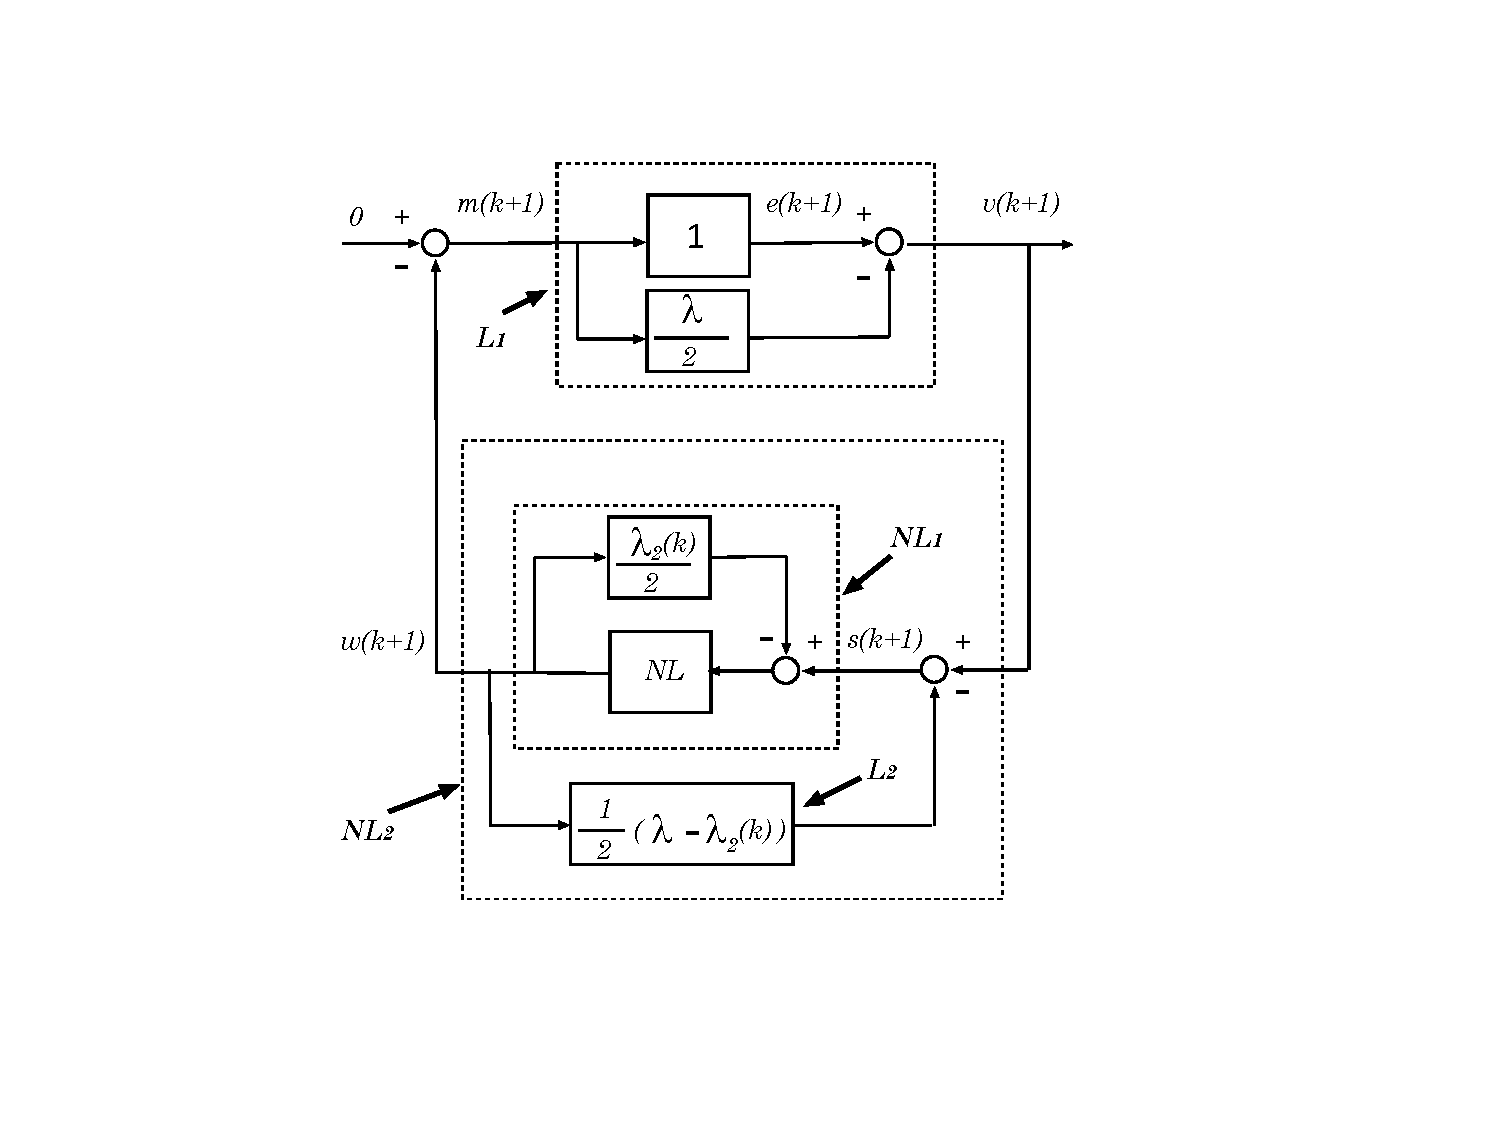
\includegraphics[width=6cm]{figs_hyperstability}\\
    \end{figure}
\end{frame}

\begin{frame}
    \frametitle{Stability theorem proof, part 1}

    We will now show that $NL_1$ is P-class:
    \begin{figure}[h]
        \centering
        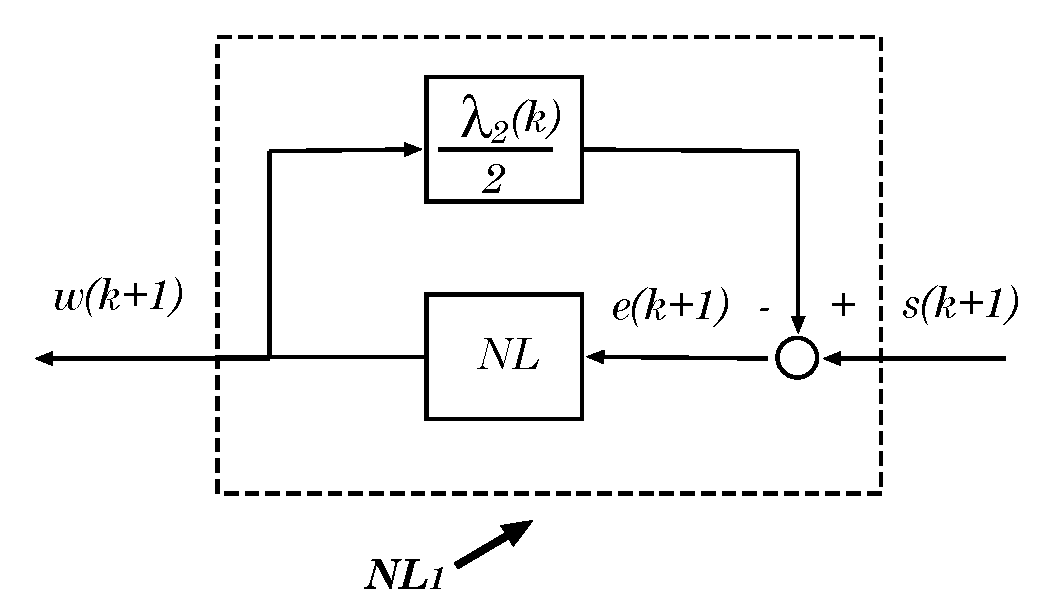
\includegraphics[width=5cm]{figs_NL1}\\
    \end{figure}
    \begin{align*}
        w(k) = -\phi^T(k-\drm) \tilde{\theta}_c(k)
    \end{align*}
    \pause

    Note that $\displaystyle e(k) = s(k) - \frac{\lambda_2(k-1)}{2} w(k)$, which implies that
    \begin{align*}
        s(k) = \frac{\lambda_2(k-1)}{2} w(k) + e(k)
    \end{align*}

\end{frame}

\begin{frame}
    \frametitle{Stability theorem proof, part 1}

    \begin{align*}
        2 w(k) s(k) & = w(k) \left[ {\color{red} \lambda_2(k-1) w(k)}
            + {\color{blue} 2 e(k)} \right] \\
        & = {\color{red} \lambda_2(k-1) \tilde{\theta}_c^T(k) \phi(k-\drm) \phi^T(k-\drm)
            \tilde{\theta}_c(k) } \\
        & \quad - {\color{blue} 2 \tilde{\theta}_c^T(k) [ \phi(k-\drm) e(k) ] } \\
        & = {\color{red} \tilde{\theta}_c^T(k) \Big[ \lambda_2(k-1) \phi(k-\drm) \phi^T(k-\drm) \Big]
            \tilde{\theta}_c(k) } \\
        & \quad - {\color{blue} 2 \tilde{\theta}_c^T(k) \left[ \lambda_1(k) F^{-1}(k-1)
            \Big( \tilde{\theta}_c(k-1) - \tilde{\theta}_c(k) \Big) \right] }
    \end{align*}
    \pause

    Define $\Delta \theta_c(k) = \hat{\theta}(k) - \hat{\theta}(k-1) = \tilde{\theta}_c(k-1) - \tilde{\theta}_c(k)$
    \pause
    \begin{align*}
        2 w(k) s(k) & = {\color{red} \tilde{\theta}_c^T(k)
            \Big[ F^{-1}(k) - \lambda_1(k) F^{-1}(k-1) \Big] \tilde{\theta}_c(k) } \\
        & \quad - {\color{blue} 2 \lambda_1(k) \tilde{\theta}_c^T(k) F^{-1}(k-1) \Delta \theta_c(k) }
    \end{align*}
\end{frame}

\begin{frame}
    \frametitle{Stability theorem proof, part 1}

    \vspace*{-\baselineskip}
    \begin{align*}
        2 w(k) s(k) & = {\color{red} \tilde{\theta}_c^T(k)
            \Big[ F^{-1}(k) - \lambda_1(k) F^{-1}(k-1) \Big] \tilde{\theta}_c(k) } \\
        & \quad - {\color{blue} 2 \lambda_1(k) \tilde{\theta}_c^T(k) F^{-1}(k-1) \Delta \theta_c(k) }
    \end{align*}
    \hrule{\hfill}
    
    \vspace*{-\baselineskip}
    \begin{align*}
        2 w(k) s(k) & = {\color{red} \tilde{\theta}_c^T(k) F^{-1}(k) \tilde{\theta}_c(k) }
            - \lambda_1(k) \Big[ {\color{red} \tilde{\theta}_c^T(k) F^{-1}(k-1) \tilde{\theta}_c(k) } \\
        & \quad {\color{blue} + 2 \tilde{\theta}_c^T(k) F^{-1}(k-1) \Delta\theta_c(k) } \Big] \\
        & = \tilde{\theta}_c^T(k) F^{-1}(k) \tilde{\theta}_c(k) \\
        & \quad - \lambda_1(k) \Big[ \Big( \tilde{\theta}_c(k) + \Delta\theta_c(k) \Big)^T
            F^{-1}(k-1) \Big( \tilde{\theta}_c(k) + \Delta\theta_c(k) \Big) \\
        & \quad - \Delta\theta_c^T(k) F^{-1}(k-1) \Delta\theta_c(k) \Big]
    \end{align*}
    \pause
    Note that $\tilde{\theta}_c(k) + \Delta \theta_c(k) = \tilde{\theta}_c(k-1)$
\end{frame}

\begin{frame}
    \frametitle{Stability theorem proof, part 1}

    From the previous slide,
    \begin{align*}
        2 w(k) s(k) & = \tilde{\theta}_c^T(k) F^{-1}(k) \tilde{\theta}_c(k)
            - \lambda_1(k) \tilde{\theta}_c^T(k-1) F^{-1}(k-1) \tilde{\theta}_c(k-1) \\
        & \quad + \lambda_1(k) \Delta\theta_c^T(k) F^{-1}(k-1) \Delta\theta_c(k)
    \end{align*}
    \pause
    
    Since $\lambda_1(k) \leq 1$ and $F(k-1) \succ 0$, this implies that
    \begin{align*}
         2 w(k) s(k) \geq \left[ \tilde{\theta}_c^T(k) F^{-1}(k) \tilde{\theta}_c(k)
            - \tilde{\theta}_c^T(k-1) F^{-1}(k-1) \tilde{\theta}_c(k-1) \right]
    \end{align*}
\end{frame}

\begin{frame}
    \frametitle{Stability theorem proof, part 1}

    \begin{align*}
         2 w(k) s(k) \geq \left[ \tilde{\theta}_c^T(k) F^{-1}(k) \tilde{\theta}_c(k)
            - \tilde{\theta}_c^T(k-1) F^{-1}(k-1) \tilde{\theta}_c(k-1) \right]
    \end{align*}
    \hrule{\hfill}
    
    Therefore
    \begin{align*}
        \Rightarrow \sum_{j=0}^k w(j) s(j) & \geq \frac{1}{2} \sum_{j=0}^k \Bigg[
            \tilde{\theta}_c^T(j) F^{-1}(j) \tilde{\theta}_c(j) \\
        & \quad - \tilde{\theta}_c^T(j-1) F^{-1}(j-1) \tilde{\theta}_c(j-1) \Bigg] \\
        & = \frac{1}{2} \Bigg[ \tilde{\theta}_c^T(k) F^{-1}(k) \tilde{\theta}_c(k)
            - \tilde{\theta}_c^T(-1) F^{-1}(-1) \tilde{\theta}_c(-1) \Bigg] \\
        & \geq - \frac{1}{2} \tilde{\theta}_c^T(-1) F^{-1}(-1) \tilde{\theta}_c(-1)
    \end{align*}
\end{frame}

\begin{frame}
    \frametitle{Stability theorem proof, part 1}

    \begin{columns}[c]
        \column{0.5\textwidth}
        We have shown that $NL_1$ is P-class

        $ \ $

        Using the same arguments as in Lecture 21 (including the asymptotic hyperstability theorem), this yields
        \alignbox{
            \lim_{k\rightarrow \infty} e(k) = 0
        }

        \column{0.5\textwidth}
        \begin{figure}[h]
            \centering
            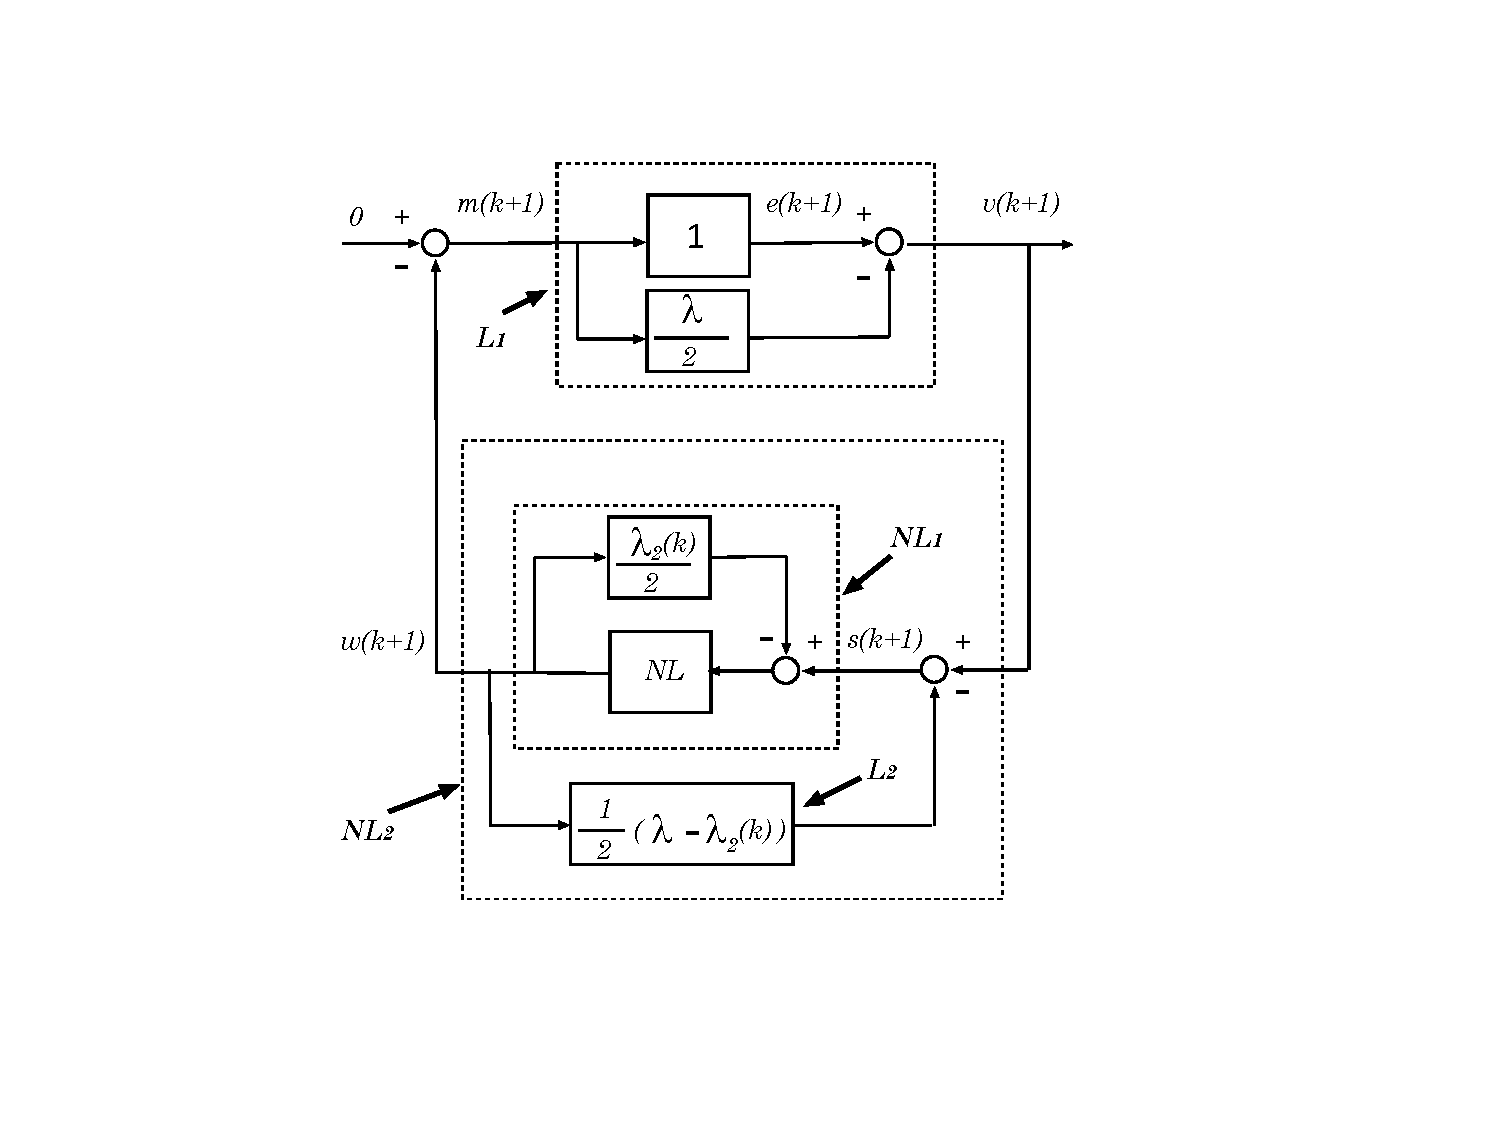
\includegraphics[width=5cm]{figs_hyperstability}\\
        \end{figure}
    \end{columns}

\end{frame}

